

\documentclass{article}[14pt, oneside, a4paper, times]

\usepackage[utf8]{inputenc}
\usepackage[english]{babel}
\usepackage[T1]{fontenc}
\usepackage{epsfig}           % para incluir figuras
\usepackage{subfig}
\usepackage{graphicx}
\usepackage{setspace}
\usepackage{vmargin}
\usepackage{algorithm}
\usepackage{algorithmic}
\usepackage{amsfonts} 
\usepackage{amssymb}


\setpapersize [portrait]{A4}
\setmarginsrb {30mm} % margem esquerda
              {10mm} % margem topo
             {30mm} % margem direita
            {20mm} % margem pé
           {2ex}  % altura do espaco para cabeçalho
           {5ex}  % espaço entre fim do cabeçalho e início do texto
          {0pt}  % altura do espaço para rodapé
         {20mm}  % espaço entre fim do texto e fim do rodapé

\doublespacing

%=======================================================================
\pagestyle{myheadings}
\begin {document}

\title{Recognising the Chilean Month Word Database}
\author{Luiz S. Oliveira and Marisa Morita  
\\
\vspace {-10pt}
Federal University of Parana (UFPR)\\
\vspace {-10pt}
Department of Informatics (DInf)\\
\vspace {-10pt}
R. Rua Cel. Francisco H. dos Santos, 100, Curitiba, PR, Brazil \\
lesoliveira@inf.ufpr.br \\ 
}


\date{}
\maketitle
%\vspace{-2\baselineskip}
\thispagestyle{empty}

%\begin{abstract}

%bla bla


%\end{abstract}

%%%%%%%%%%%%%%%%%%%%%%%%%%%%%%%%%%%%%%%%%%%%%%%%%%%%%%%%%%%%%%%%%%%%%%%%%%%%%%%%%
% Introduction 
%%%%%%%%%%%%%%%%%%%%%%%%%%%%%%%%%%%%%%%%%%%%%%%%%%%%%%%%%%%%%%%%%%%%%%%%%%%%%%%%%
\section{Introduction} 

In this report we describe the results of the experiments performed on the Chilean month word database. It is worth of remark that this dataset still is under construction, therefore the number of samples still is limited and not all the classes are available. To overcome these limitations, we have performed the recognition using the models trained with the Brazilian month words. Before presenting the recognition results, we present the preprocessing steps performed to remove baselines, background, and some noise.

\section{Pre-processing}

The pre-processing used so far is composed of three basic steps. First we convert the 256-graylevel image to a binary image using Otsu algorithm. We have tried out some other methods but Otsu seems to produce the best results. The second step is devoted to remove the baseline, which usually is located in the bottom but also may appear anywhere in the image. Some different strategies were tried out in this case, such as the morphological opening, but the by searching and removing for very long and thin components seems to be a good alternative. The final step intends to remove salt-and-pepper noise resulting from the binarization processes. This is done through a median filter of size 3. Figure \ref{samples:fig} shows some examples of the database before and after the pre-processing. One possible solution for this kind of problem could be a strategy based on adaptive thresholding.  


 \begin {figure} [htb]
    \centering
    \mbox
        {
        \subfloat[] {
\epsfig {file=enero1, width=4cm}}\quad 
        \subfloat[] {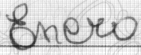
\epsfig {file=enero2, width=4cm}}\quad 
        \subfloat[] {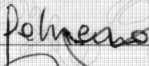
\epsfig {file=febrero1, width=4cm}} 
        }
       \mbox
        {
        \subfloat[] {
\epsfig {file=enero1bin, width=4cm}}\quad 
        \subfloat[] {
\epsfig {file=enero2bin, width=4cm}}\quad 
        \subfloat[] {
\epsfig {file=febrero1bin, width=4cm}} 
        }
       
    \caption{Some examples extracted from the database and their corresponding binary images.}
    \label{samples:fig}
\end{figure}

Im most cases the pre-processing produces good results. In some cases, though, specially when the pressure on the handwriting is weak, some parts of the image are lost. This is exemplified in Figure \ref{missing:fig}. In this case, it can be noticed that the baseline stroke is quite stronger than the handwriting itself. This has an important impact in the binarization process. 


 \begin {figure} [htb]
    \centering
    \mbox
        {
        \subfloat[] {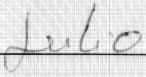
\epsfig {file=julio1, width=4cm}}\quad 
        \subfloat[] {
\epsfig {file=julio1bin, width=4cm}}
        }
         
    \caption{Some examples extracted from the database and their corresponding binary images.}
    \label{missing:fig}
\end{figure}

\section{Recognition Results}

Based on our previous results (reported in Report \#3), the best results using global features 
were achieved by the parallel model (Figure \ref{paralel-models:fig}), in which the 12 HMM word models are built by concatenating all the corresponding characters. For this reason we decided to employ this model in this first experiment with the Chilean month word database. 

\begin{figure}[htbp]
   \centering
   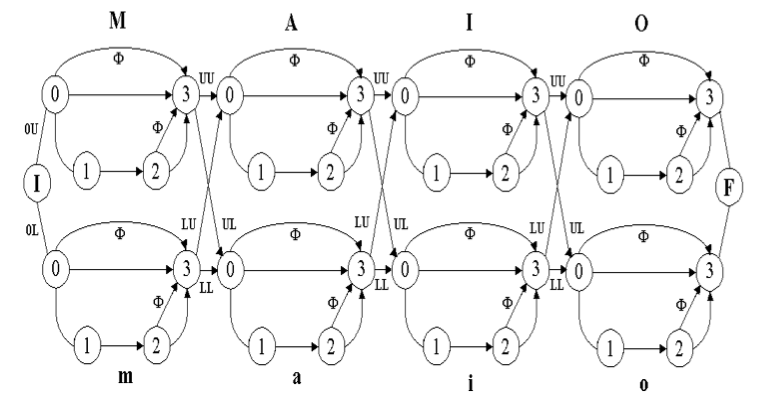
\epsfig{file=paralel-models, width=14cm}
   \caption{Training model of class ``Maio''}
   \label{paralel-models:fig}
\end{figure}

Independently of the architecture choice, the first challenge to overcome is the lack of some characters in the training set. As stated before, as we do not have enough data, we have used the Brazilian database to train the models. However, the Brazilian database does not have the characters ``y'' (appearing in Mayo) and ``p'' (appearing in Septiembre). in the 12 months. Since we are relying on Global features, we tried to find similar characters to replace those missing. To replace ``y'' and ``p'', we have used ``j'' and ``g'', respectively. In both cases, we have selected characters with descenders. This may work for cursive characters, but for upper-case this replacement is not straightforward.  

Other aspect that compromises the performance on this database is the presence of spurious segments coming from other parts of the bank cheques. This kind of problem, which is illustrated in Figure \ref{spurious:fig}, is a by-product of the segmentation and may have an impact in the feature extraction, hence, in the classification. A more elaborated pre-processing or segmentation strategy would be necessary to deal with this kind of problem. 

 \begin {figure} [htb]
    \centering
    \mbox
        {
        \subfloat[] {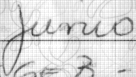
\epsfig {file=junio1, width=4cm}}\quad 
        \subfloat[] {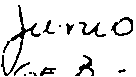
\epsfig {file=junio1bin, width=4cm}}
        }
         
    \caption{Segmentation problems.}
    \label{spurious:fig}
\end{figure}


We have performed the recognition of about 800 words available in the Chilean month word database. The recognition results for TOP1 and TOP3 are 42.2\% and 74.7\%, respectively. The confusion matrices for TOP1 and TOP3 are presented in Tables \ref{top1:tab} and \ref{top3:tab}, respectively. 


\begin{table} [ht!]
\caption {Confusion Matrix (\%) - TOP1}
\begin{center}
\begin{tabular}{rrrrrrrrrr} \hline 
 \multicolumn{1}{c}{Class}&
 \multicolumn{1}{c}{1}&
 \multicolumn{1}{c}{2}&
 \multicolumn{1}{c}{3}&
 \multicolumn{1}{c}{4}&
 \multicolumn{1}{c}{5}&
 \multicolumn{1}{c}{6}&
 \multicolumn{1}{c}{7}&
 \multicolumn{1}{c}{8}&
 \multicolumn{1}{c}{9} \\ \hline

1 & \textbf{42.9}	&	19.8	&	3.3	 &	4.4	&	2.2	&	18.7&	6.6	&	2.2	&	0.0 \\
2 & 14.9	&	\textbf{57.4}	&	7.4	 &	4.3	&	0.0	&	5.3	&	5.3	&	2.1	&	3.2\\
3 & 32.6	&	21.1	&	\textbf{22.1} &	1.1	&	6.3	&	10.5&	1.1	&	5.3	&	0.0\\
4 & 38.9	&	14.7	&	4.2	 &	\textbf{27.4}&	1.1	&	3.2	&	5.3	&	4.2	&	1.1\\
5 & 22.9	&	6.3	    &	22.9 &	1.0	&	\textbf{35.4}&	8.3	&	2.1	&	1.0	&	0.0\\
6 & 14.4	&	12.4	&	2.1	 &	1.0	&	1.0	&	\textbf{60.8}&	8.2	&	0.0	&	0.0\\
7 & 19.0	&	9.0	    &	1.0	 &	1.0	&	1.0	&	12.0&	\textbf{57.0}&	0.0	&	0.0\\
8 & 17.2	&	21.2	&	4.0	 &	10.1&	3.0	&	3.0	&	5.1	&	\textbf{31.3}&	5.1\\
9 & 0.0	    &	11.8	&	5.9	 &	11.8&	0.0	&	0.0	&	0.0	&	11.8&	\textbf{58.8}\\ \hline

\end{tabular}
\label{top1:tab}
\end{center}
\end{table}




\begin{table} [ht!]
\caption {Confusion Matrix (\%) - TOP3}
\begin{center}
\begin{tabular}{rrrrrrrrrr} \hline 
 \multicolumn{1}{c}{Class}&
 \multicolumn{1}{c}{1}&
 \multicolumn{1}{c}{2}&
 \multicolumn{1}{c}{3}&
 \multicolumn{1}{c}{4}&
 \multicolumn{1}{c}{5}&
 \multicolumn{1}{c}{6}&
 \multicolumn{1}{c}{7}&
 \multicolumn{1}{c}{8}&
 \multicolumn{1}{c}{9} \\ \hline

1 & \textbf{68.1}	&	14.3&	3.3	&	3.3	&	1.1	&	5.5	&	3.3	&	1.1	&	0.0\\
2 & 12.8	&	\textbf{76.6}&	3.2	&	2.1	&	0.0	&	2.1	&	1.1	&	1.1	&	1.1\\
3 & 12.6	&	8.4	&	\textbf{66.3}&	0.0	&	2.1	&	9.5	&	1.1	&	0.0	&	0.0\\
4 & 22.1	&	4.2	&	4.2	&	\textbf{61.1}	&	0.0	&	3.2	&	3.2	&	1.1	&	1.1\\
5 & 15.6	&	3.1	&	2.1	&	1.0	&	\textbf{70.8}	&	5.2	&	1.0	&	1.0	&	0.0\\
6 & 7.2 	&	3.1	&	1.0	&	1.0	&	1.0	&	\textbf{86.6}	&	0.0	&	0.0	&	0.0\\
7 & 3.0 	&	4.0	&	1.0	&	1.0	&	1.0	&	0.0	&	\textbf{90.0}	&	0.0	&	0.0\\
8 & 8.1 	&	7.1	&	2.0	&	3.0	&	1.0	&	2.0	&	3.0	&	\textbf{72.7}	&	1.0\\
9 & 0.0 	&	0.0	&	0.0	&	0.0	&	0.0	&	0.0	&	0.0	&	0.0	&	\textbf{100.0}\\ \hline

\end{tabular}
\label{top3:tab}
\end{center}
\end{table}

\section{Concluding Remarks}

As we may observe, the results are considerable lower than the results presented on the Brazilian dataset. It is not necessary to mention that the Brazilian database, in spite of all variability it presents, is a laboratory database. In other words, a worst performance was expected for the Chilean database. We believe, however, that the performance can be increased when more data become available. Then we can retrain the HMM models considering all characters appearing in the Chilean month words and also make the models absorb some of the variability of the Chilean writing style. In the meanwhile, we will extract other features (concavity-based) and use them in a multiple-codebook strategy.



%The source code is available in the SVN repository. Before compiling the code make sure to update the \textsf{PPROJ} variable in the \textsf{Make\_orand\_globfeat} file available in the directory \textsf{./tools/orand/batch/feature/gen} and also to update the defines in the \textsf{global.h} file, available in the directory \textsf{./tools/orand/inter/include}. To compile the source code use

%\begin{verbatim}
%make -f Make_orand_globfeat
%\end{verbatim}

%\noindent And to execute the program, type

%\begin{verbatim}
%./orand_globfeat feat1 globf
%\end{verbatim}

%The program generates three different files for training, validation and testing, respectively. Those files are located in the directory \textsf{./tools/orand/param/train/feat1} and \textsf{./tools/orand/param/test/feat1}.



%\begin{figure}[htbp]
%   \centering
%   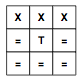
\epsfig{file=mask, width=2.5cm}
%   \caption{3 $\times$ 3 mask used for smoothing.}
%   \label{mask:fig}
%\end{figure}


\bibliographystyle{IEEEbib}
\bibliography{refer}



\end{document}



